\qrchapter{https://forgottenpillar.com/rsc/en-fp-chapter14}{Adventist pioneers and the Trinity doctrine}


\qrchapter{https://forgottenpillar.com/rsc/en-fp-chapter14}{Los pioneros adventistas y la doctrina trinitaria}


Sister White wrote that early Adventist pioneers \egwinline{are to bear their testimony as to what constitutes the truth for this time}[Lt329-1905.18; 1905][https://egwwritings.org/read?panels=p8455.24] because \egwinline{they have learned to avoid errors and dangers, and are they not then competent to give wise counsel}[7T 287.3; 1902][https://egwwritings.org/read?panels=p117.1637]? In their writings, we see their unanimous views regarding the \emcap{personality of God}, and that they have avoided the Trinitarian error. There is much to write about this topic because the Adventist pioneers left a lot of material dealing directly or indirectly with the doctrine of Trinity. But we will look at some of the testimonies from James White and brother Loughborough because we have read some of their articles on the \emcap{personality of God}. Also, we will compare their testimony with the Spirit of Prophecy as we have done so far.


La hermana White escribió que los primeros pioneros adventistas \egwinline{deben dar su testimonio en cuanto a lo que constituye la verdad para este tiempo}[Lt329-1905.18; 1905][https://egwwritings.org/read?panels=p8455.24] porque \egwinline{han aprendido a evitar los errores y los peligros, y ¿no son entonces competentes para dar un sabio consejo}[7T 287.3; 1902][https://egwwritings.org/read?panels=p117.1637]? En sus escritos, vemos sus puntos de vista unánimes respecto a la \emcap{personalidad de Dios}, y que han evitado el error trinitario. Hay mucho que escribir sobre este tema porque los pioneros adventistas dejaron mucho material que trata directa o indirectamente de la doctrina trinitaria. Pero veremos algunos de los testimonios de James White y del hermano Loughborough porque hemos leído algunos de sus artículos sobre la \emcap{personalidad de Dios}. Además, compararemos sus testimonios con el Espíritu de Profecía como hemos hecho hasta ahora.


James White, in the Review and Herald, listed \others{some of \textbf{the popular fables} of the age}”, saying: “\others{Here we might mention \textbf{the Trinity, which \underline{does away the personality of God, and of his Son Jesus Christ,} }and of sprinkling or pouring instead of being ‘buried with Christ in baptism,’ ‘planted in the likeness of his death:’ but we pass from these \textbf{fables }to notice one that is held sacred by nearly all professed Christians, both Catholic and Protestant. It is, the change of the Sabbath of the fourth commandment from the seventh to the first day of the week.}[James S. White, Review \& Herald, December 11, 1855, p. 85.15][http://documents.adventistarchives.org/Periodicals/RH/RH18551211-V07-11.pdf]


James White, en la Review and Herald, enumeró \others{algunas de \textbf{las fábulas populares} de la época}”, diciendo: “\others{Aquí podríamos mencionar \textbf{la Trinidad, que \underline{elimina la personalidad de Dios, y de su Hijo Jesucristo,} }y de rociar o derramar en lugar de ser ‘sepultado con Cristo en el bautismo’, ‘plantado en la semejanza de su muerte:’ pero pasamos de estas \textbf{fábulas }para notar una que es considerada sagrada por casi todos los cristianos profesos, tanto católicos como protestantes. Es, el cambio del sábado del cuarto mandamiento del séptimo al primer día de la semana.}[James S. White, Review \& Herald, December 11, 1855, p. 85.15][http://documents.adventistarchives.org/Periodicals/RH/RH18551211-V07-11.pdf]


What does James White mean when he says that the Trinity \others{does away with the personality of God, and of his Son Jesus Christ}? In Day Star, he wrote:


¿Qué quiere decir James White cuando dice que la Trinidad \others{elimina la personalidad de Dios, y de su Hijo Jesucristo}? En Day Star, escribió:


\others{…a certain class who \textbf{deny the only Lord God and our Lord Jesus Christ}. This class can be no other than those who \textbf{spiritualize away the existence of the Father and the Son}, \textbf{as \underline{two distinct}, \underline{literal}, \underline{tangible persons}}, also a literal Holy city and throne of David… The way spiritualizers this way have disposed of or \textbf{denied the only Lord God and our Lord Jesus Christ is first using \underline{the old unscriptural trinitarian creed}}, viz, that Jesus Christ is the eternal God, though they have not one passage to support it, while we have plain scripture testimony in abundance \textbf{that He is the Son of the eternal God.}}[James White, Day Star, Jan 24, 1846][https://m.egwwritings.org/en/book/741.25\#27]


\others{...una cierta clase que \textbf{niega al único Señor Dios y a nuestro Señor Jesucristo}. Esta clase no puede ser otra que aquellos que \textbf{espiritualizan la existencia del Padre y del Hijo}, \textbf{como \underline{dos}, \underline{literales}, \underline{tangibles personas}}, también una literal ciudad santa y trono de David... La forma en que los espiritualizadores han dispuesto o \textbf{negado al único Señor Dios y a nuestro Señor Jesucristo es primero usando \underline{el antiguo credo trinitario no bíblico}}, es decir, que Jesucristo es el Dios eterno, aunque no tienen ni un pasaje para apoyarlo, mientras que nosotros tenemos testimonio bíblico claro en abundancia \textbf{que Él es el Hijo del Dios eterno.}}[James White, Day Star, Jan 24, 1846][https://m.egwwritings.org/en/book/741.25\#27]


Doing away with the personality of God and His Son is accomplished by denying Them as two distinct, literal, and tangible persons. The doctrine on the personality of God teaches that the Father has a literal, \textit{tangible} person.


Eliminar la personalidad de Dios y de Su Hijo se logra negándolos como dos personas distintas, literales y tangibles. La doctrina sobre la personalidad de Dios enseña que el Padre tiene una persona literal, \textit{tangible}.


In the Adventist Review and Sabbath Herald article from April 4, 1854, James White listed 10 points of \textit{Catholic reasons for keeping Sunday}”, where he said that the Sunday \others{is a day dedicated by the apostles to \textbf{the honor of the most Holy Trinity}}[The Advent Review, and Sabbath Herald, vol. 5 April 4, 1854, p. 86][https://egwwritings.org/read?panels=p1643.2867]. Here we also see the harmony between J. B. Frisbie and James White in their view that the Sabbath is dedicated to the biblical God expressed in the first point of the \emcap{Fundamental Principles}, and Sunday is dedicated to the trinity God. The main problem with the Trinity doctrine is that it \others{does away the personality of God, and of his Son Jesus Christ}. In Life Incidents, he wrote more about why this is so.


En el artículo de la Adventist Review and Sabbath Herald del 4 de abril de 1854, James White enumeró 10 puntos de \textit{razones católicas para guardar el domingo}”, donde dijo que el domingo \others{es un día dedicado por los apóstoles al \textbf{honor de la Santísima Trinidad}}[The Advent Review, and Sabbath Herald, vol. 5 April 4, 1854, p. 86][https://egwwritings.org/read?panels=p1643.2867]. Aquí también vemos la armonía entre J. B. Frisbie y James White en su opinión de que el sábado está dedicado al Dios bíblico expresado en el primer punto de los \emcap{Principios Fundamentales}, y el domingo está dedicado al dios trinitario. El principal problema con la doctrina trinitaria es que \others{elimina la personalidad de Dios, y de su Hijo Jesucristo}. En Life Incidents, escribió más sobre por qué es así.


\others{\textbf{Jesus prayed that his disciples might be one as he was \underline{one with his Father}}. \textbf{This prayer did not contemplate one disciple with twelve heads, but twelve disciples, made one in object and effort in the cause of their Master}. \textbf{\underline{Neither are the Father and the Son parts of the ‘three-one God.}}’\footnote{The same quotation is found in James White’s book “\textit{The Law and the Gospel}” with one difference. He states, “\textit{Neither are the Father and the Son parts of \underline{one being}}”; in “\textit{Life Incidents}”, he wrote “parts of the ‘\underline{three-one God}’”. See \href{https://egwwritings.org/?ref=en_LAGO.1.2&para=1492.10}{James S. White, The Law and the Gospel p. 1.2}.} \textbf{\underline{They are two distinct beings}}, \textbf{yet one in the design and accomplishment of redemption}. The redeemed, from the first who shares in the great redemption, to the last, all ascribe the honour, and glory, and praise, of their salvation, to \textbf{both God and the Lamb}.}[James S. White, Life Incidents, p.343.2][https://egwwritings.org/read?panels=p1462.1743]


\others{\textbf{Jesús oró para que sus discípulos fueran uno como él era \underline{uno con su Padre}}. \textbf{Esta oración no contemplaba un discípulo con doce cabezas, sino doce discípulos, hechos uno en objeto y esfuerzo en la causa de su Maestro}. \textbf{\underline{Tampoco el Padre y el Hijo son partes del ‘Dios tres-en-uno.}}’\footnote{La misma cita se encuentra en el libro de James White “\textit{The Law and the Gospel}” con una diferencia. Él afirma, “\textit{Tampoco el Padre y el Hijo son partes de \underline{un ser}}”; en “\textit{Life Incidents}”, escribió “partes del ‘\underline{Dios tres-en-uno}’“. Ver \href{https://egwwritings.org/?ref=en_LAGO.1.2&para=1492.10}{James S. White, The Law and the Gospel p. 1.2}.} \textbf{\underline{Son dos seres distintos}}, \textbf{pero uno en el designio y la realización de la redención}. Los redimidos, desde el primero que participa en la gran redención, hasta el último, atribuyen el honor, la gloria y la alabanza de su salvación, \textbf{tanto a Dios como al Cordero}.}[James S. White, Life Incidents, p.343.2][https://egwwritings.org/read?panels=p1462.1743]


Sister White wrote similarly regarding Christ’s prayer:


La hermana White escribió algo similar con respecto a la oración de Cristo:


\egw{The burden of that prayer was that His disciples might be \textbf{one as He was one with the Father}; the oneness so close that, \textbf{although \underline{two distinct beings}}, there was \textbf{perfect unity of spirit, purpose, and action}. The mind of the Father was the mind of the Son.}[Lt1-1882.1; 1882][https://egwwritings.org/read?panels=p4120.5]


\egw{El peso de esa oración era que sus discípulos fueran \textbf{uno como Él era uno con el Padre}; la unidad era tan estrecha que, \textbf{aunque \underline{dos seres distintos}}, había \textbf{perfecta unidad de espíritu, propósito y acción}. La mente del Padre era la mente del Hijo.}[Lt1-1882.1; 1882][https://egwwritings.org/read?panels=p4120.5]


\egw{\textbf{The unity that exists between Christ and His disciples \underline{does not destroy the personality of either}}. They are one in purpose, in mind, in character, \textbf{but \underline{not in person}}. \textbf{It is thus that God and Christ are one}.}[MH, 421 422; 1905][https://egwwritings.org/read?panels=p135.2177]


\egw{\textbf{La unidad que existe entre Cristo y sus discípulos \underline{no destruye la personalidad de ninguno de ellos}}. Son uno en propósito, en mente, en carácter, \textbf{pero \underline{no en persona}}. \textbf{Es así que Dios y Cristo son uno}.}[MH, 421 422; 1905][https://egwwritings.org/read?panels=p135.2177]


The Father and the Son do not comprise one person nor being. The Father and the Son are one, just as Christ and His disciples are one—one in spirit, purpose, mind, and character.


El Padre y el Hijo no constituyen una persona ni un ser. El Padre y el Hijo son uno, así como Cristo y sus discípulos son uno—uno en espíritu, propósito, mente y carácter.


Many Adventist trinitarian scholars charge James White and other early pioneers for arianism or semi-arianism, claiming that they made Christ inferior to the Father. This is not true. Let us read the testimony of James White on this matter.


Muchos eruditos trinitarios adventistas acusan a James White y a otros pioneros de arrianismo o semiarrianismo, afirmando que hicieron a Cristo inferior al Padre. Esto no es cierto. Leamos el testimonio de James White sobre este asunto.


\others{Paul affirms of \textbf{the Son of God that he was in the form of God}, and that \textbf{\underline{he was equal with God}}. ‘\textbf{Who being in the form of God thought it not robbery to be \underline{equal with God}}.’ Phil. 2:6. The reason why it is not robbery for the Son \textbf{to be equal with the Father is the fact that he is equal}. If the Son is not equal with the Father, then it is robbery for him to rank himself with the Father.}


\others{Pablo afirma del \textbf{Hijo de Dios que era en forma de Dios}, y que \textbf{\underline{era igual a Dios}}. ‘\textbf{El cual, siendo en forma de Dios, no consideró el ser \underline{igual a Dios} como un robo}.’ Fil. 2:6. La razón por la que no es un robo que el Hijo \textbf{sea igual al Padre es el hecho de que es igual}. Si el Hijo no es igual al Padre, entonces es un robo que se clasifique con el Padre.}


\othersnogap{\textbf{\underline{The inexplicable trinity that makes the godhead three in one and one in three, is bad enough}}; \textbf{but that ultra Unitarianism that makes Christ inferior to the Father is worse}. Did God say to an inferior, Let us make man in our image?’}[James S. White, The Advent Review and Sabbath Herald, November 29, 1877, p. 171][https://documents.adventistarchives.org/Periodicals/RH/RH18771129-V50-22.pdf]


\othersnogap{\textbf{\underline{La inexplicable trinidad que hace a la divinidad tres en uno y uno en tres, ya es suficientemente mala}}; \textbf{pero ese ultra unitarismo que hace a Cristo inferior al Padre es peor}. ¿Acaso dijo Dios a un inferior: Hagamos al hombre a nuestra imagen?’}[James S. White, The Advent Review and Sabbath Herald, November 29, 1877, p. 171][https://documents.adventistarchives.org/Periodicals/RH/RH18771129-V50-22.pdf]


The problem of the Adventist trinitarian scholars lies in that they themselves cannot completely explain Christ’s divinity other than through the Trinitarian paradigm. Adventist pioneers did believe in Christ’s full divinity but they rejected the Trinity because it destroys the \emcap{personality of God}. \others{The inexplicable trinity that makes the godhead three in one and one in three, \textbf{is bad enough}}. Below is another statement from James White where he compared Seventh-day Adventist with Seventh-day Baptist belief. Seventh-day Adventists did not believe in the Trinity unlike Seventh-day Baptists. James White mentioned that, regarding the divinity of Christ, Seventh-day Adventists hold so nearly with the trinitarian Seventh-day Baptists that they apprehend no trial there.


El problema de los eruditos trinitarios adventistas radica en que ellos mismos no pueden explicar completamente la divinidad de Cristo más que a través del paradigma trinitario. Los pioneros adventistas sí creían en la plena divinidad de Cristo, pero rechazaban la Trinidad porque destruye la \emcap{personalidad de Dios}. \others{La inexplicable trinidad que hace que la divinidad sea tres en uno y uno en tres, \textbf{es suficientemente mala}}. A continuación hay otra declaración de James White donde comparó la creencia adventista del séptimo día con la bautista del séptimo día. Los adventistas del séptimo día no creían en la Trinidad, a diferencia de los bautistas del séptimo día. James White mencionó que, en lo que respecta a la divinidad de Cristo, los adventistas del séptimo día están tan cerca de los bautistas del séptimo día trinitarios, que no ven ningún juicio al respecto.


\others{\textbf{The principal difference between the two bodies is the immortality question}. \textbf{The S. D. Adventists hold \underline{the divinity of Christ so nearly with the trinitarian}, that we apprehend no trial here}. And as the practical application of the subject of the Gifts of the Spirit to our people and to our work is better understood by our S. D. Baptist brethren, they manifest less concern for us on this account.}[James S. White, The Advent Review and Sabbath Herald, October 12, 1876, p. 116][https://documents.adventistarchives.org/Periodicals/RH/RH18761012-V48-15.pdf]


\others{\textbf{La principal diferencia entre los dos cuerpos es la cuestión de la inmortalidad}. \textbf{Los Adventistas del S. D. sostienen \underline{la divinidad de Cristo de manera tan cercana a los trinitarios}, que no aprehendemos ningún juicio aquí}. Y como la aplicación práctica del tema de los Dones del Espíritu a nuestro pueblo y a nuestra obra es mejor comprendida por nuestros hermanos bautistas del S. D., ellos manifiestan menos preocupación por nosotros por este motivo.}[James S. White, The Advent Review and Sabbath Herald, October 12, 1876, p. 116][https://documents.adventistarchives.org/Periodicals/RH/RH18761012-V48-15.pdf]


This evidence should raise questions to each Adventist trinitarian scholar. How could it be that the Adventist pioneers adhere to the divinity of Christ as trinitarians did, yet rejected the Trinity doctrine? In which way was Christ fully divine, if He was not part of an amalgamated three-in-one God? The answer is simple and completely Biblical. Christ is fully divine, just as His Father, because He was begotten in the express image of the Father’s person; thus, He inherited complete divine nature from His Father.


Esta evidencia debería plantear preguntas a cada erudito trinitario adventista. ¿Cómo es posible que los pioneros adventistas se adhirieron a la divinidad de Cristo como lo hacían los trinitarios y, sin embargo, rechazaron la doctrina trinitaria? ¿En qué sentido era Cristo plenamente divino, si no formaba parte de un Dios amalgamado tres en uno? La respuesta es sencilla y completamente bíblica. Cristo es plenamente divino, al igual que su Padre, porque fue engendrado a la imagen expresa de la persona del Padre; por lo tanto, heredó la naturaleza divina completa de su Padre.


\egw{A complete offering has been made; for ‘God so loved the world, that he gave his only-begotten Son,’—\textbf{not a son by creation}, as were the angels, nor a son by adoption, as is the forgiven sinner, but \textbf{a Son \underline{begotten} in the express image of the Father’s person}, and in all the brightness of his majesty and glory, \textbf{one equal with God} in authority, dignity, and \textbf{divine perfection}. \textbf{In him dwelt all the fullness of the Godhead bodily}.}[ST May 30, 1895, par. 3; 1895][https://egwwritings.org/read?panels=p820.12891]


\egw{Se ha hecho una ofrenda completa; porque ‘tanto amó Dios al mundo, que dio a su Hijo unigénito,’—\textbf{no un hijo por creación}, como lo fueron los ángeles, ni un hijo por adopción, como lo es el pecador perdonado, sino \textbf{un Hijo \underline{engendrado} a la imagen expresa de la persona del Padre}, y en todo el resplandor de su majestad y gloria, \textbf{uno igual a Dios} en autoridad, dignidad, y \textbf{perfección divina}. \textbf{En él habitaba toda la plenitud de la Divinidad corporalmente}.}[ST May 30, 1895, par. 3; 1895][https://egwwritings.org/read?panels=p820.12891]


Christ's complete divinity is not based on an amalgamated \emcap{personality of God}, but rather on His Sonship with the Father. The Bible never refers to Christ with the term “\textit{one God}”—only the Father is referred to with the term “\textit{one God}”\footnote{John 17:3; 1. Corinthians 8:6; 1. Timothy 2:5; Ephesians 4:6} \footnote{We study Christ’s complete divinity in-depth  in the second book of the Forgotten Pillar Project - “\textit{Rediscovering the Pillar}”}. Jesus, the Son of God, is fully divine but is not referred to as \others{\textbf{one God}, \textbf{a personal, spiritual being}} in the first point of the \emcap{Fundamental Principles}.


La divinidad completa de Cristo no se basa en una \emcap{personalidad} amalgamada de Dios, sino en su filiación con el Padre. La Biblia nunca se refiere a Cristo con el término “\textit{un Dios}”—sólo se refiere al Padre con el término “\textit{un Dios}”\footnote{Juan 17:3; 1. Corintios 8:6; 1. Timoteo 2:5; Efesios 4:6} \footnote{Estudiamos la divinidad completa de Cristo en profundidad en el segundo libro del Proyecto Pilar Olvidado - “\textit{Redescubriendo el Pilar}”}. Jesús, el Hijo de Dios, es plenamente divino pero no se refiere a él como \others{\textbf{un Dios}, \textbf{un ser personal y espiritual}} en el primer punto de los \emcap{Principios Fundamentales}.


\egw{The Lord Jesus Christ, the only begotten Son of the Father, \textbf{is truly God in infinity, \underline{but not in personality}}.}[Ms116-1905.19; 1905][https://egwwritings.org/read?panels=p10633.25]


\egw{El Señor Jesucristo, el único Hijo engendrado del Padre, \textbf{es verdaderamente Dios en infinidad, \underline{pero no en personalidad}}.}[Ms116-1905.19; 1905][https://egwwritings.org/read?panels=p10633.25]


Brother J. N. Loughborough was asked to answer the question, \others{What serious objection is there to the doctrine of the Trinity?}[The question was asked by Brother W. W. Giles and it was sent to James S. White, who forwarded the question to Brother John N. Loughborough.]. As we read his answer, let us try to understand some of the reasons why the early pioneers did not adhere to this doctrine.


Al hermano J. N. Loughborough se le pidió que respondiera a la pregunta, \others{¿Qué objeción seria hay a la doctrina de la trinidad?}[La pregunta fue formulada por el hermano W. W. Giles y fue enviada a James S. White, quien remitió la pregunta al hermano John N. Loughborough.]. Al leer su respuesta, tratemos de comprender algunas de las razones por las que los primeros pioneros no se adhirieron a esta doctrina.


\others{There are many objections which we might urge, but on account of our limited space we shall reduce them to the three following: \textbf{1. It is contrary to common sense. 2. It is contrary to scripture. 3. Its origin is Pagan and fabulous.}}


\others{Son muchas las objeciones que podríamos plantear, pero debido a nuestro limitado espacio las reduciremos a las tres siguientes: \textbf{1. Es contraria al sentido común. 2. Es contraria a las escrituras. 3. Su origen es pagano y fabuloso.}}


\othersnogap{These positions we will remark upon briefly in their order. And 1. \textbf{It is not very consonant with common sense to talk of three being one, and one being three}. \textbf{Or as some express it, calling God ‘the Triune God,’ or ‘the three-one-God.’} \textbf{If Father, Son, and Holy Ghost are each God, it would be three Gods; for three times one is not one, but three}. \textbf{\underline{There is a sense in which they are one, but not one person, as claimed by Trinitarians}}}.


\othersnogap{Estas posiciones las comentaremos brevemente en su orden. Y 1. \textbf{No es muy consonante con el sentido común hablar de que tres son uno, y uno es tres}. \textbf{O como algunos lo expresan, llamar a Dios ‘el Dios trino’, o ‘el Dios tres-uno’.} \textbf{Si el Padre, el Hijo y el Espíritu Santo son cada uno Dios, serían tres dioses; porque tres veces uno no es uno, sino tres}. \textbf{\underline{Hay un sentido en el que son uno, pero no una persona, como afirman los trinitarios}}}.


\othersnogap{2. \textbf{It is contrary to Scripture}. \textbf{Almost any portion of the New Testament we may open which has occasion to speak of the Father and Son, represents them as two distinct persons}. \textbf{\underline{The seventeenth chapter of John is alone sufficient to refute the doctrine of the Trinity}}. \textbf{Over forty times in that one chapter Christ speaks of his Father as a person distinct from himself}. His Father was in heaven and he upon earth. The Father had sent him. Given to him those that believed. He was then to go to the Father.\textbf{ And in this very testimony he shows us in what consists the oneness of the Father and Son}.\textbf{\underline{ It is the same as the oneness of the members of Christ’s church}}. ‘\textbf{That \underline{they} all may be one; \underline{as} thou, Father, art in me, and I in thee, \underline{that they also} may be one in us}; that the world may believe that thou hast sent me. And the \textbf{glory which thou gavest me I have given them}; that \textbf{they may be one}, \textbf{even as we are one.}’ \textbf{Of one heart and one mind}. \textbf{Of one purpose} in all the plan devised for man’s salvation. \textbf{\underline{Read the seventeenth chapter of John, and see if it does not completely upset the doctrine of the Trinity}}.}


\othersnogap{2. \textbf{Es contrario a las escrituras}. \textbf{Casi cualquier parte del Nuevo Testamento que podamos abrir y que tenga ocasión de hablar del Padre y del Hijo, los representa como dos personas distintas}. \textbf{\underline{El capítulo diecisiete de Juan es suficiente para refutar la doctrina de la trinidad}}. \textbf{En ese capítulo, Cristo habla más de cuarenta veces de su Padre como una persona distinta de él}. Su Padre estaba en el cielo y él en la tierra. El Padre lo había enviado. Le dio a los que creyeron. Él debía entonces ir al Padre.\textbf{ Y en este mismo testimonio nos muestra en qué consiste la unidad del Padre y del Hijo}.\textbf{\underline{ Es lo mismo que la unidad de los miembros de la iglesia de Cristo}}. ‘\textbf{Para que \underline{ellos} todos sean uno; \underline{como} tú, Padre, estás en mí, y yo en ti, \underline{que también ellos} sean uno en nosotros}; para que el mundo crea que tú me has enviado. Y la \textbf{gloria que me diste, yo se la he dado a ellos}; para que \textbf{sean uno}, \textbf{como nosotros somos uno.}’ \textbf{De un solo corazón y una sola mente}. \textbf{De un solo propósito} en todo el plan ideado para la salvación del hombre. \textbf{\underline{Leed el capítulo diecisiete de Juan, y ved si no desbarata por completo la doctrina de la trinidad}}.}


\othersnogap{\textbf{To believe that doctrine, when reading the scripture we must believe that God sent himself into the world, died to reconcile the world to himself, raised himself from the dead, ascended to himself in heaven, pleads before himself in heaven to reconcile the world to himself, and is the only mediator between man and himself}. It will not do to substitute the human nature of Christ (according to Trinitarians) as the Mediator; for Clarke says, ‘Human blood can no more appease God than swine’s blood.’ Comment on 2 Samuel 21:10. \textbf{We must believe also that in the garden God prayed to himself, if it were possible, to let the cup pass from himself, and a thousand other \underline{such absurdities}}.}


\othersnogap{\textbf{Para creer esa doctrina, al leer la escritura debemos creer que Dios se envió a sí mismo al mundo, murió para reconciliar al mundo consigo mismo, resucitó de entre los muertos, ascendió a sí mismo en el cielo, aboga ante sí mismo en el cielo para reconciliar al mundo consigo mismo, y es el único mediador entre el hombre y él mismo}. No sirve sustituir la naturaleza humana de Cristo (según los trinitarios) como mediador; porque Clarke dice: ‘La sangre humana no puede apaciguar a Dios más que la sangre de cerdo’. Comentario sobre 2 Samuel 21:10. \textbf{Debemos creer también que en el jardín Dios se rogó a sí mismo, si era posible, que dejara pasar la copa de sí mismo, y mil otros \underline{absurdos} semejantes}.}


\othersnogap{\textbf{Read carefully the following texts, comparing them with the idea that Christ is the Omnipotent, Omnipresent, Supreme, and only self-existent God: John 14:28; 17:3; 3:16; 5:19, 26; 11:15; 20:19; 8:50; 6:38; Mark 13:32; Luke 6:12; 22:69; 24:29; Matthew 3:17; 27:46; Galatians 3:20; 1 John 2:1; Revelation 5:7; Acts 17:31. Also see Matthew 11:25, 27; Luke 1:32; 22:42; John 3:35, 36; 5:19, 21, 22, 23, 25, 26; 6:40; 8:35, 36; 14:13; 1 Corinthians 15:28, etc}.}


\othersnogap{\textbf{Lee cuidadosamente los siguientes textos, comparándolos con la idea de que Cristo es el Dios Omnipotente, Omnipresente, Supremo y único auto existente: Juan 14:28; 17:3; 3:16; 5:19, 26; 11:15; 20:19; 8:50; 6:38; Marcos 13:32; Lucas 6:12; 22:69; 24:29; Mateo 3:17; 27:46; Gálatas 3:20; 1 Juan 2:1; Apocalipsis 5:7; Hechos 17:31. Véase también Mateo 11:25, 27; Lucas 1:32; 22:42; Juan 3:35, 36; 5:19, 21, 22, 23, 25, 26; 6:40; 8:35, 36; 14:13; 1 Corintios 15:28, etc}.}


\othersnogap{\textbf{The word Trinity nowhere occurs in the Scriptures}. \textbf{The principal text supposed to teach it is 1 John 1:7\footnote{J. N. Loughborough made a typo in the original document, he wanted to point out to 1 John 5:7}, which is an interpolation}. Clarke says, ‘\textbf{Out of one hundred and thirteen manuscripts, the text is wanting in one hundred and twelve. It occurs in no MS. before the tenth century. And the first place the text occurs in Greek, is in the Greek translation of the acts of the Council of Lateran, held A. D. 1215}.’ - Comment. on John 1, and remarks at close of chap.}


\othersnogap{\textbf{La palabra trinidad no aparece en ninguna parte de las escrituras}. \textbf{El principal texto que se supone que la enseña es 1 Juan 1:7\footnote{J. N. Loughborough cometió un error tipográfico en el documento original, quería señalar 1 Juan 5:7}, que es una interpolación}. Clarke dice: ‘\textbf{De ciento trece manuscritos, el texto falta en ciento doce. No aparece en ningún manuscrito anterior al siglo X. Y el primer lugar en el que aparece el texto en griego es en la traducción griega de las actas del concilio de Letrán, celebrado en 1215}’. - Comentario sobre Juan 1 y observaciones al final del capítulo.}


\othersnogap{3. \textbf{Its origin is pagan and fabulous}. Instead of pointing us to scripture for proof of the trinity, we are pointed to the trident of the Persians, with the assertion that by this they designed to teach the idea of a trinity, and if they had the doctrine of the trinity, they must have received it by tradition from the people of God. \textbf{But this is all assumed, for it is certain that the Jewish church held to no such doctrine. Says Mr. Summerbell, ‘A friend of mine who was present in a New York synagogue, asked the Rabbi for an explanation of the \underline{word ’elohim’}. A Trinitarian clergyman who stood by, replied, ‘Why, that has \underline{reference to the three persons in the Trinity},’ when a Jew stepped forward and said he must not mention that word again, or they would have to compel him to leave the house; \underline{for it was not permitted to mention the name of any strange god in the synagogue}.’}\footnote{Discussion between Summerbell and Flood on Trinity, p.38.} Milman says the idea of the Trident is fabulous. (Hist. Christianity, p.34.)}


\othersnogap{3. \textbf{Su origen es pagano y fabuloso}. En lugar de señalarnos la escritura como prueba de la trinidad, se nos señala el tridente de los persas, con la afirmación de que con ello pretendían enseñar la idea de una trinidad, y si tenían la doctrina de la trinidad, debían haberla recibido por tradición del pueblo de Dios. \textbf{Pero todo esto es una suposición, pues es cierto que la iglesia judía no sostenía tal doctrina. Dice el señor Summerbell: ‘Un amigo mío que estaba presente en una sinagoga de Nueva York, pidió al rabino una explicación de la \underline{palabra ‘elohim’}. Un clérigo trinitario que se encontraba allí, respondió: ‘Bueno, eso se refiere a las \underline{tres personas de la trinidad}’, cuando un judío se adelantó y dijo que no debía mencionar esa palabra de nuevo, o tendrían que obligarle a salir de la casa; \underline{porque no estaba permitido mencionar el nombre de ningún dios extraño en la sinagoga}.’}\footnote{Discussion between Summerbell and Flood on Trinity, p.38.} Milman dice que la idea del Tridente es fabulosa. (Hist. Christianity, p.34.)}


\othersnogap{\textbf{This doctrine of the trinity was brought into the church about the same time with image worship, and keeping the day of the sun, and is but Persian doctrine remodeled}. \textbf{It occupied about three hundred years from its introduction to bring the doctrine to what it is now. It was commenced about 325 A. D., and was not completed till 681.} See Milman’s Gibbon’s Rome, vol. iv, p.422. It was adopted in Spain in 589, in England in 596, in Africa in 534. - Gib. vol. iv, pp.114,345; Milner, vol. i, p.519.}[John N. Loughborough, The Adventist Review, and Sabbath Herald, November 5, 1861, p. 184][https://egwwritings.org/read?panels=p1685.6615]


\othersnogap{\textbf{Esta doctrina de la trinidad fue introducida en la iglesia más o menos al mismo tiempo que la adoración de imágenes, y el mantenimiento del día del sol, y no es más que la doctrina persa remodelada}. \textbf{Desde su introducción se tardó unos trescientos años en llevar la doctrina a lo que es ahora. Se inició alrededor del año 325 d.C., y no se completó hasta el año 681.} Ver Gibbon's Rome de Milman, vol. iv, p.422. Se adoptó en España en 589, en Inglaterra en 596, en África en 534. - Gib. vol. iv, pp.114,345; Milner, vol. i, p.519.}[John N. Loughborough, The Adventist Review, and Sabbath Herald, November 5, 1861, p. 184][https://egwwritings.org/read?panels=p1685.6615]


Brother Loughborough was the son of a Methodist minister and he was raised with the belief in the doctrine of Trinity. Besides the reasons he mentioned, he does not adhere to this doctrine because it is not in harmony with the truth on the \emcap{personality of God}. The seventeenth chapter of John is in harmony with the truth on the \emcap{personality of God} taught and practiced by the Seventh-day Adventists; the Trinity doctrine is not.


El hermano Loughborough era hijo de un ministro metodista y fue educado con la creencia en la doctrina de la Trinidad. Además de las razones que mencionó, no se adhiere a esta doctrina porque no está en armonía con la verdad sobre la \emcap{personalidad de Dios}. El capítulo diecisiete de Juan está en armonía con la verdad sobre la \emcap{personalidad de Dios} enseñada y practicada por los Adventistas del Séptimo Día; la doctrina trinitaria no lo está.


\begin{figure}[hp]
    \centering
    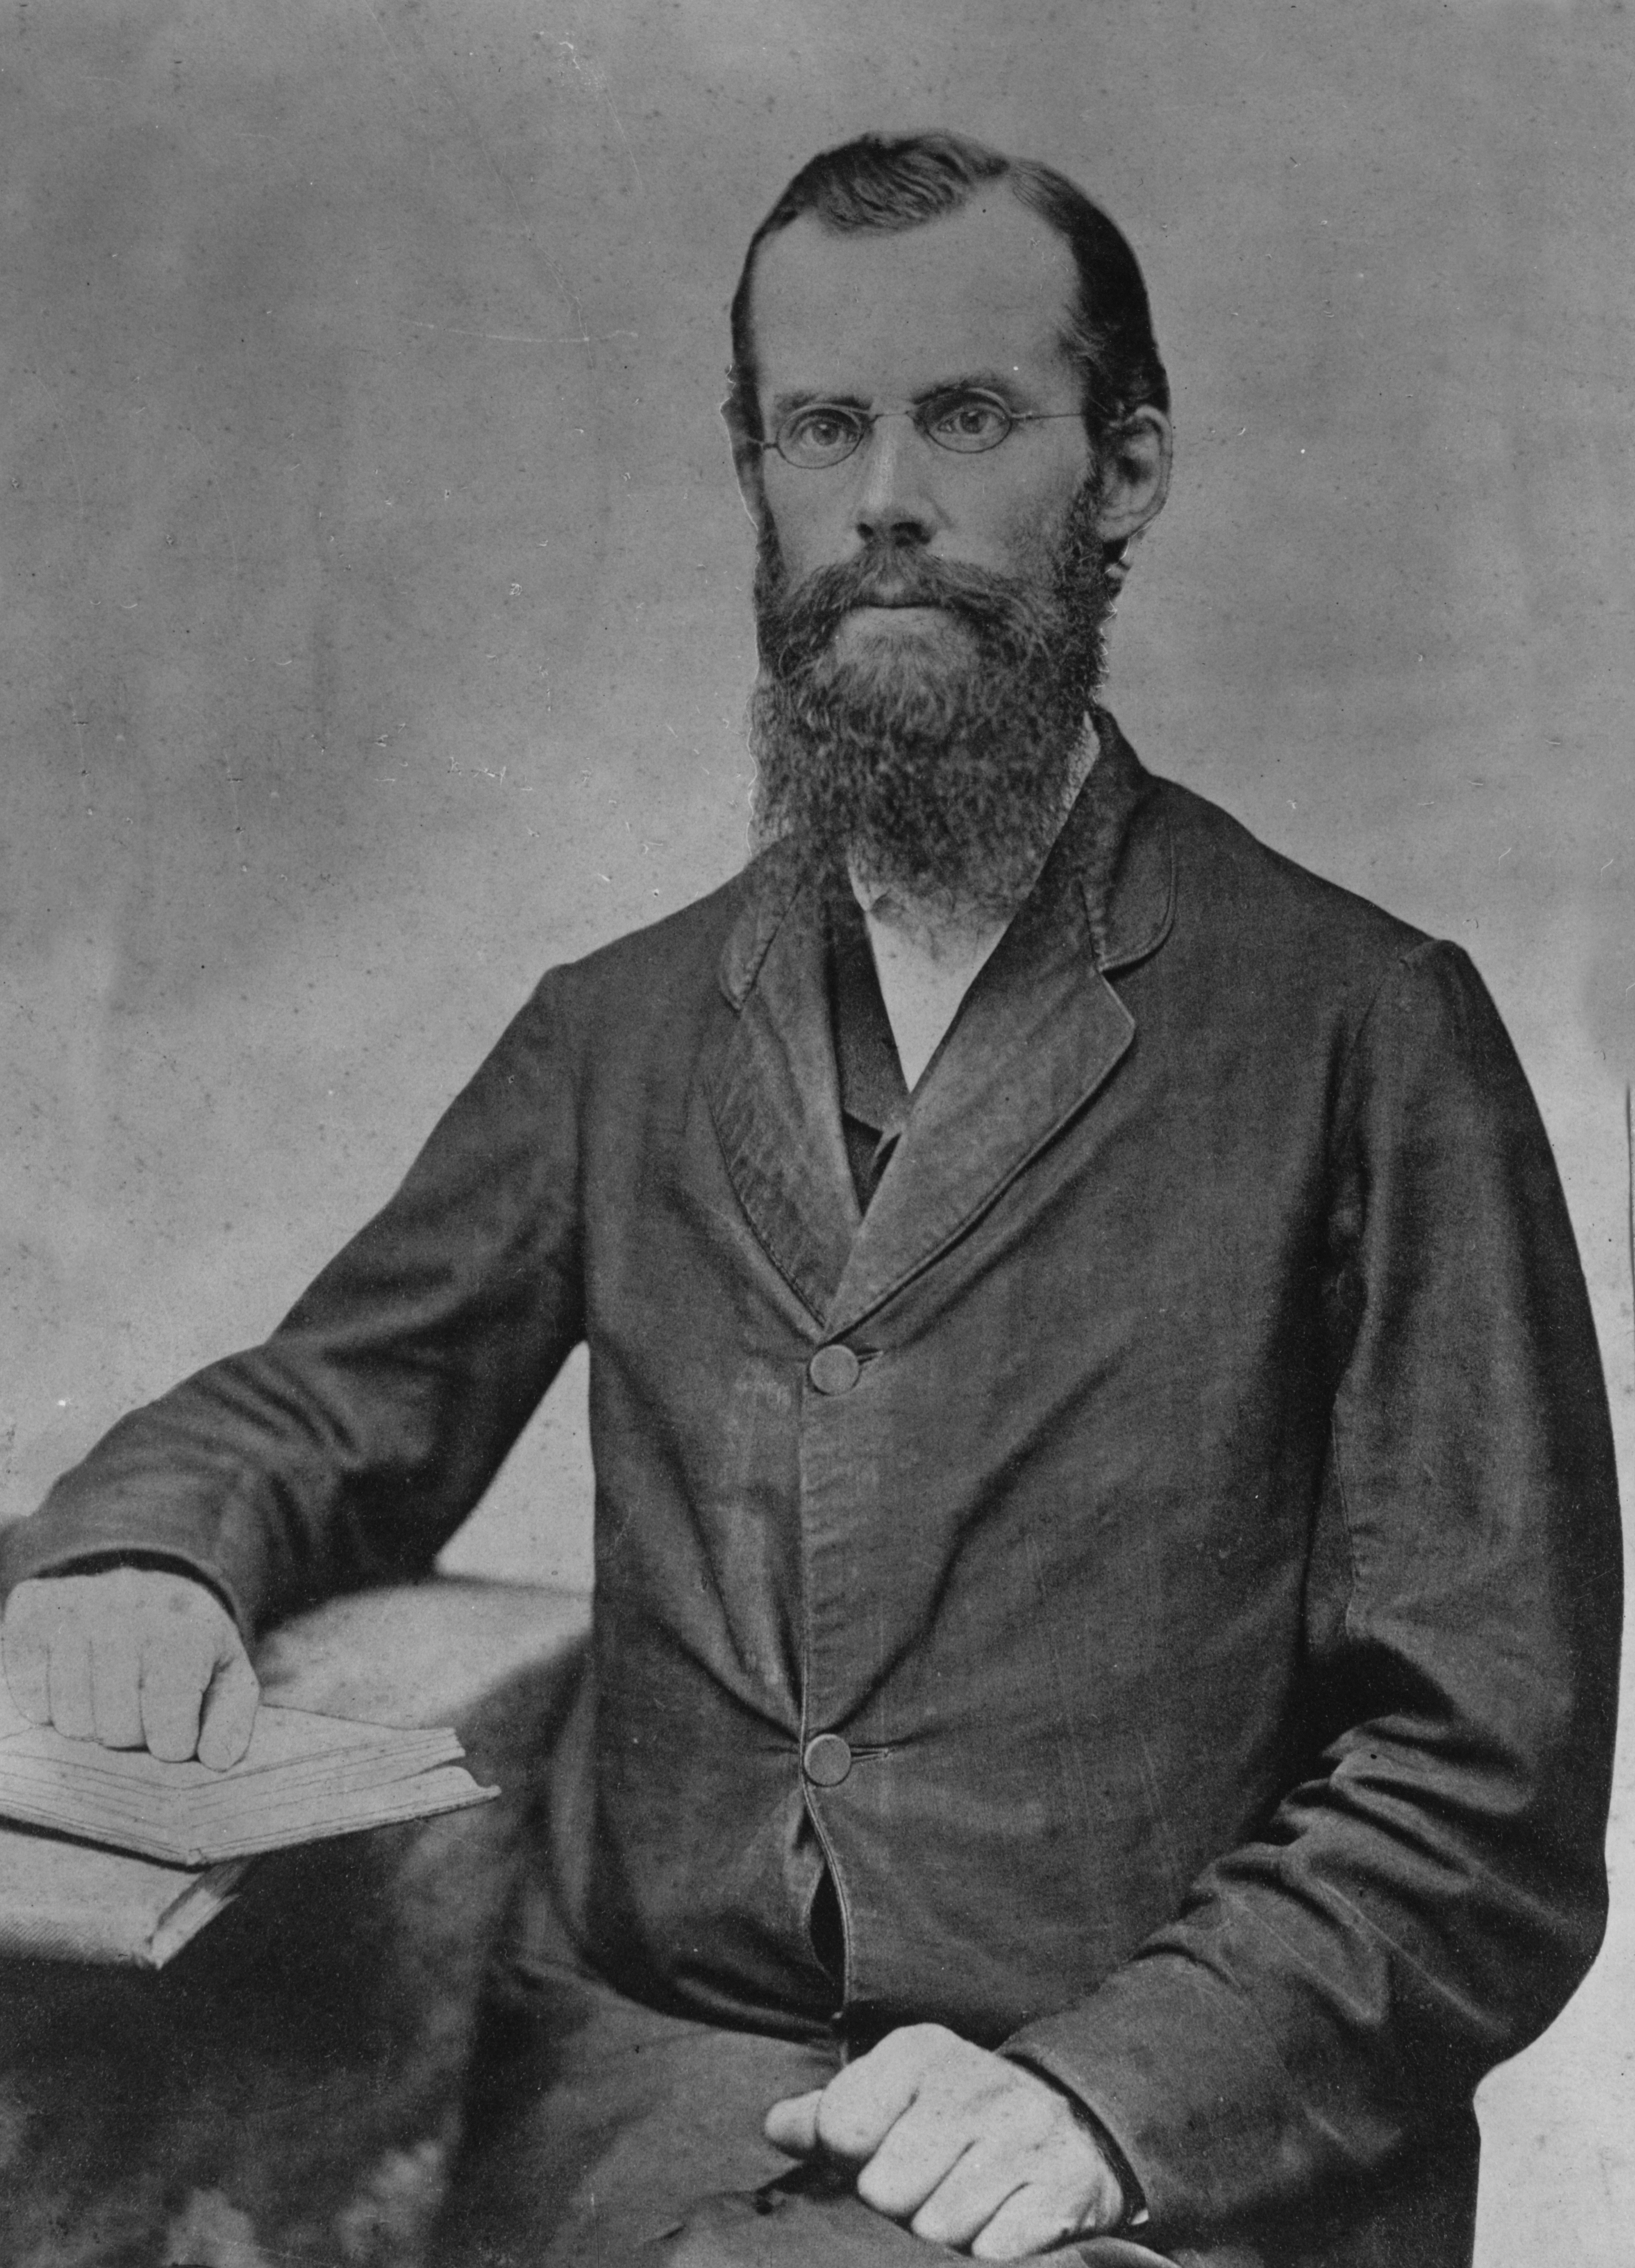
\includegraphics[width=1\linewidth]{images/john-nevins-andrews.jpg}
    \caption*{John Nevins Andrews (1829-1883)}
    \label{fig:j-n-andrews}
\end{figure}


\begin{figure}[hp]
    \centering
    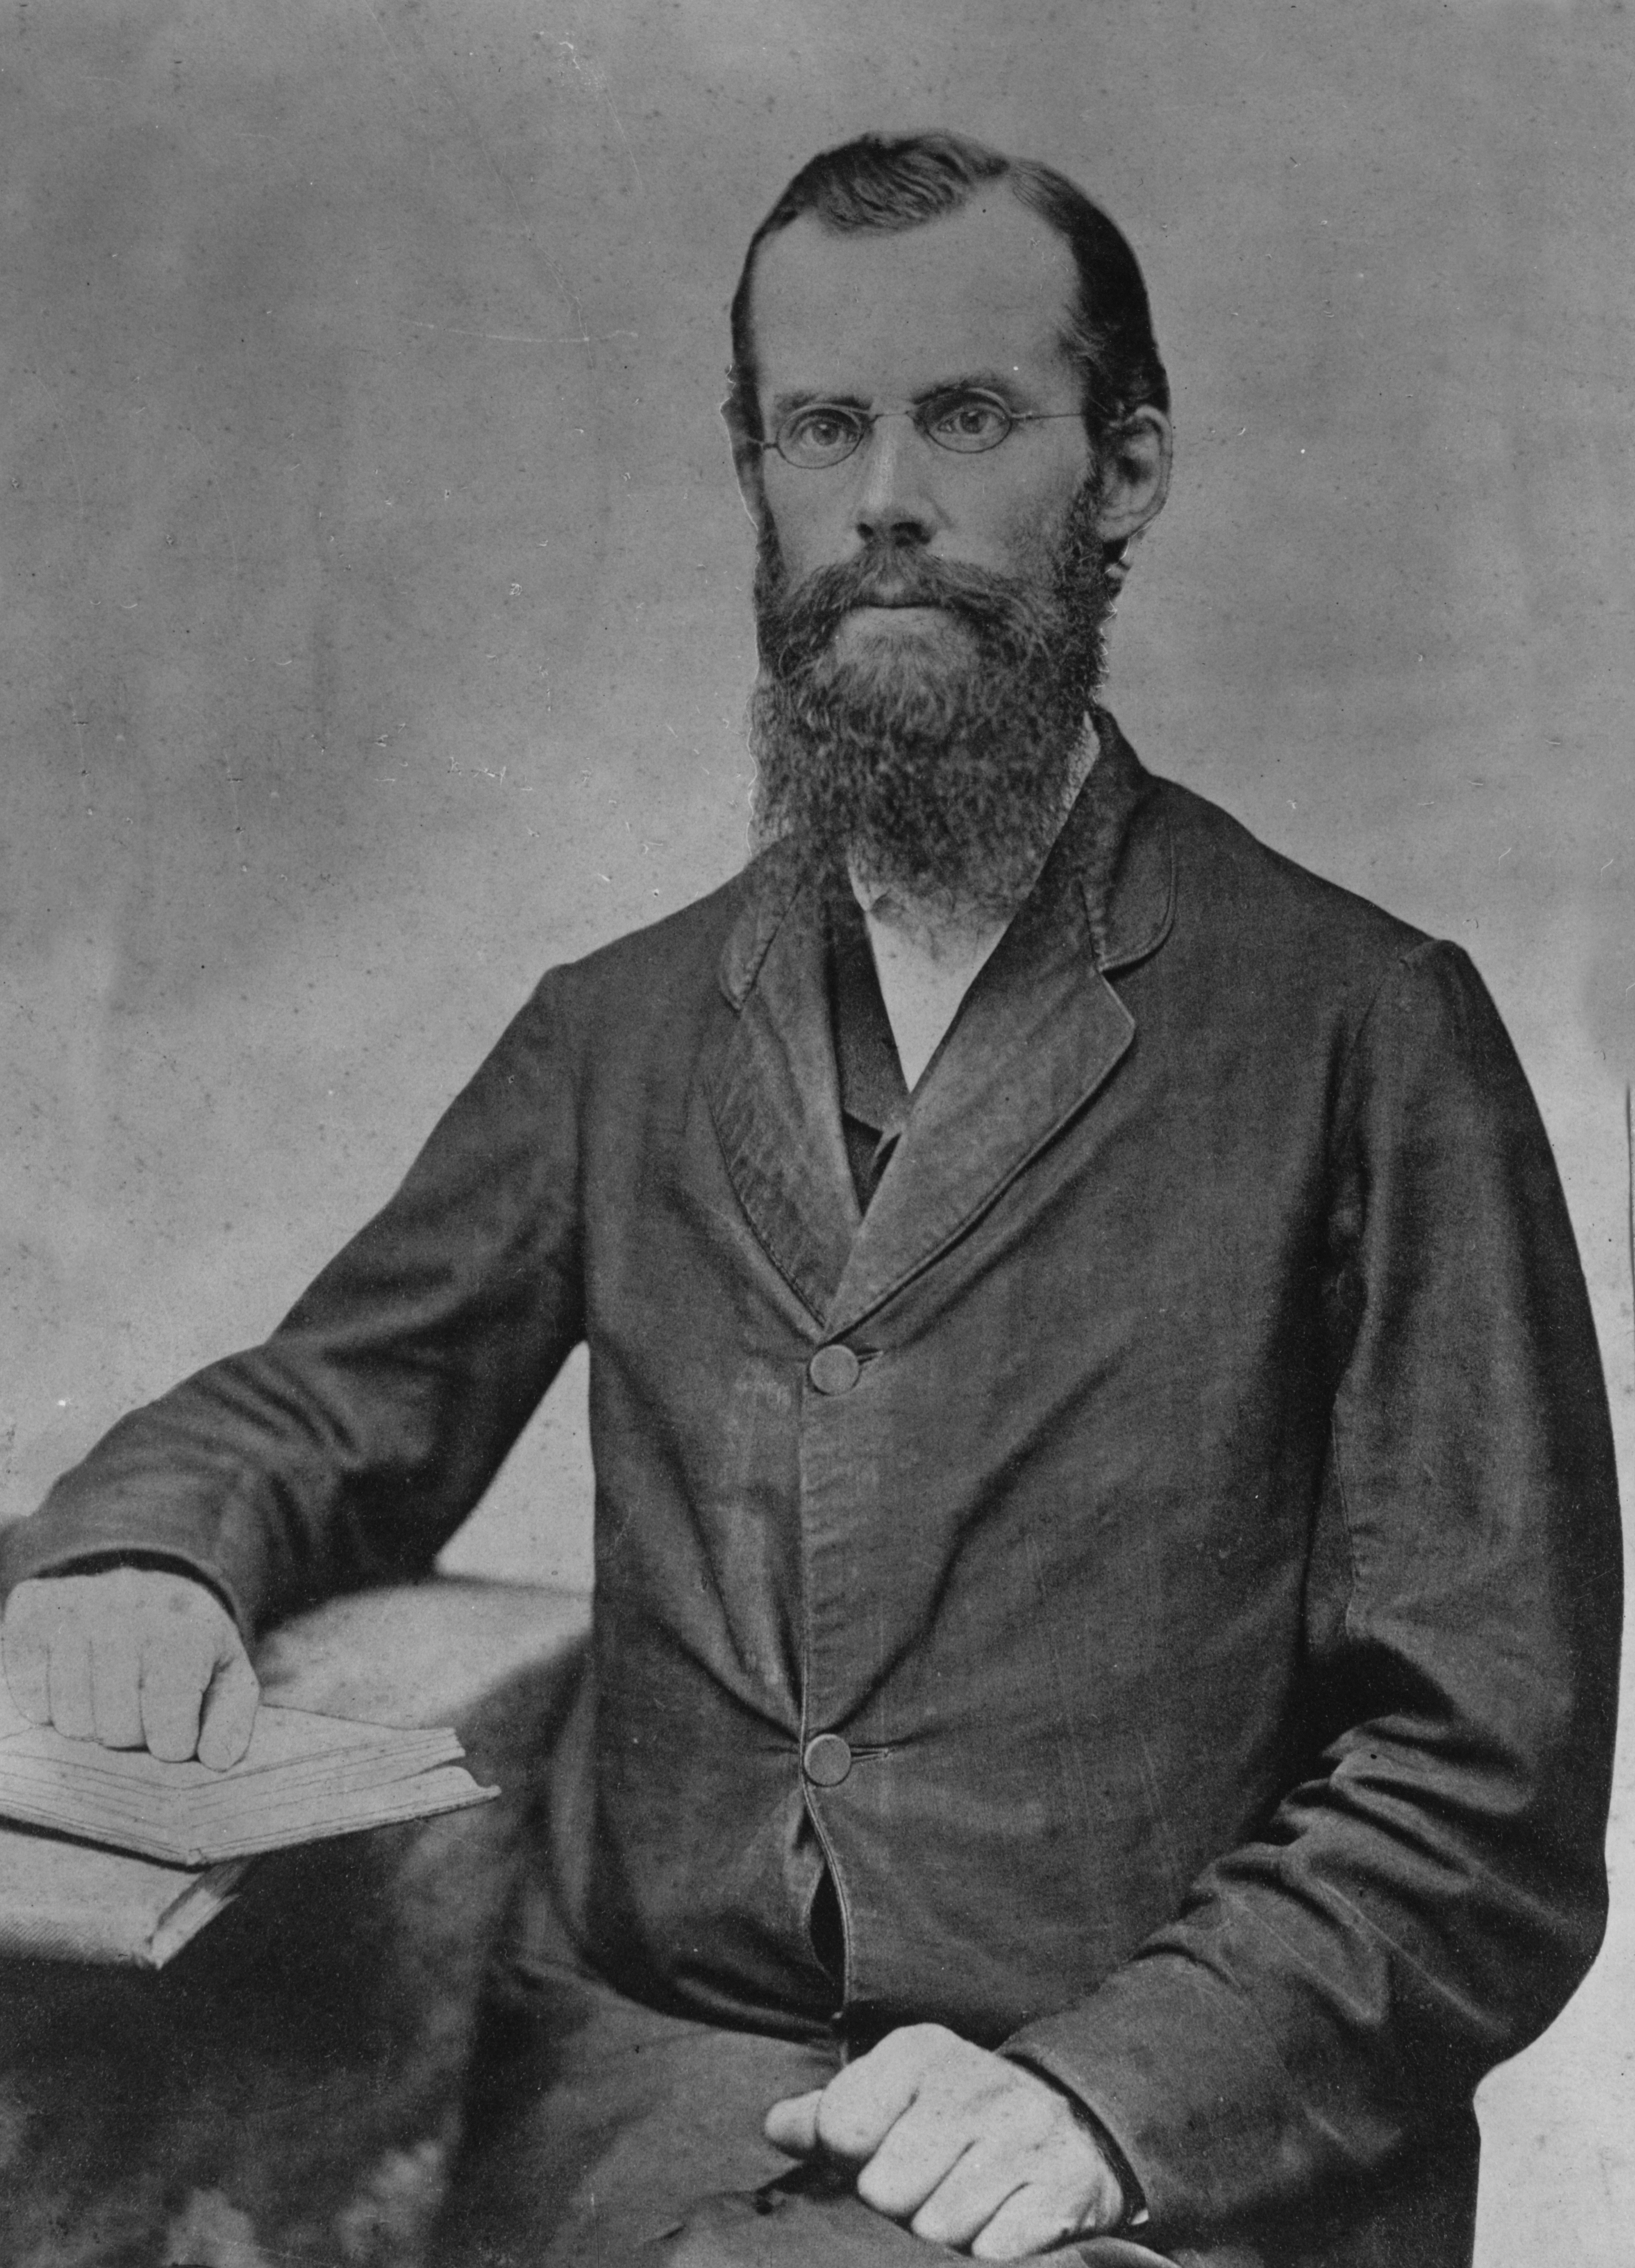
\includegraphics[width=1\linewidth]{images/john-nevins-andrews.jpg}
    \caption*{John Nevins Andrews (1829-1883)}
    \label{fig:j-n-andrews}
\end{figure}


J. N. Andrews said, \others{\textbf{The doctrine of the Trinity which was established in the church by the council of Nicea, A. D. 325}. \textbf{This doctrine \underline{destroys the personality of God, and his Son Jesus Christ our Lord}}...}[John. N. Andrews, The Advent Review and Sabbath Herald, March 6, 1855, p. 185][http://documents.adventistarchives.org/Periodicals/RH/RH18550306-V06-24.pdf]


J. N. Andrews dijo, \others{\textbf{La doctrina de la trinidad que fue establecida en la iglesia por el concilio de Nicea, el año 325 d.C.}. \textbf{Esta doctrina \underline{destruye la personalidad de Dios, y de su Hijo Jesucristo nuestro Señor}}...}[John. N. Andrews, The Advent Review and Sabbath Herald, March 6, 1855, p. 185][http://documents.adventistarchives.org/Periodicals/RH/RH18550306-V06-24.pdf]


In the context of the trinitarian understanding of the \emcap{personality of God}, it is safe to say that the \emcap{personality of God}, or the quality or state of God being a person, in any understanding of Trinity doctrine is a mystery. The problem is that there is no clear view of who is that \textit{one God} who is a person? The underlying claim is made that God is One yet Three, or One in Three; yes, God is a person, and He is one, yet simultaneously He is three persons. This view can never hold any clear perception of the \emcap{personality of God}. Also, it will deny the clearest testimony of the Scriptures that the one God is the Father, and that Christ is truly His only begotten Son. Most trinitarian brothers would agree that Christ is a real and definite being but if a trinitarian were to accept the Father as a real and definite Being, he would also need to accept the Holy Spirit as a real and definite being, thus denying the Holy Spirit as being a \textit{spirit}, the means by which the Father and Son are omnipresent. Conversely, if a trinitarian accepted the Holy Spirit to be a literal spirit, having no body nor form, then he would deny the Father to be a real, definite being. In conversation over the quality or state of God being a person, there is never a clear view of the matter with promoters of the Trinity doctrine; it is subterfuge. \textit{‘Subterfuges’} is a word Sister White used to describe the deception by artifice or stratagem in order to conceal, escape, or evade\footnote{\href{https://www.merriam-webster.com/dictionary/subterfuges}{The Merriam-Webster, ‘subterfuges’} - “\textit{deception by artifice or stratagem in order to conceal, escape, or evade}”} the truth; in other words, something that you cannot grab by head or tail. This is the primary reason Sister White did not engage in the Trinity discussion that would come up in the Seventh-day Adventist Church.


En el contexto de la comprensión trinitaria de la \emcap{personalidad de Dios}, es seguro decir que la \emcap{personalidad de Dios}, o la cualidad o estado de Dios siendo una persona, en cualquier comprensión de la doctrina trinitaria es un misterio. El problema es que no hay una visión clara de quién es ese \textit{un Dios} que es una persona. La afirmación subyacente es que Dios es Uno y a la vez Tres, o Uno en Tres; sí, Dios es una persona, y es uno, pero simultáneamente es tres personas. Este punto de vista nunca puede sostener ninguna percepción clara de la \emcap{personalidad de Dios}. Además, negará el testimonio más claro de las Escrituras de que el único Dios es el Padre, y que Cristo es verdaderamente su Hijo unigénito. La mayoría de los hermanos trinitarios estarían de acuerdo en que Cristo es un ser real y definido, pero si un trinitario aceptara al Padre como un Ser real y definido, también tendría que aceptar al Espíritu Santo como un ser real y definido, negando así que el Espíritu Santo sea un \textit{espíritu}, el medio por el cual el Padre y el Hijo son omnipresentes. Por el contrario, si un trinitario aceptara que el Espíritu Santo es un espíritu literal, que no tiene cuerpo ni forma, entonces negaría que el Padre sea un ser real y definido. En la conversación sobre la cualidad o estado de Dios siendo una persona, nunca hay una visión clara del asunto con los promotores de la doctrina trinitaria; es un subterfugio. \textit{‘Subterfugios’} es una palabra que la hermana White utilizó para describir el engaño por medio de artificios o estratagemas con el fin de ocultar, escapar o evadir\footnote{\href{https://www.merriam-webster.com/dictionary/subterfuges}{The Merriam-Webster, ‘subterfuges’} - “\textit{deception by artifice or stratagem in order to conceal, escape, or evade}”} la verdad; en otras palabras, algo que no se puede agarrar por la cabeza o la cola. Esta es la razón principal por la que la hermana White no se involucró en la discusión sobre la Trinidad que surgiría en la Iglesia Adventista del Séptimo Día.


\egw{I was cautioned not to enter into controversy \textbf{regarding the question} that \textbf{\underline{will come up}} over \textbf{these things, because controversy \underline{might lead men to resort to subterfuges, and their minds would be led away from the truth of the Word of God to assumption and guesswork}}. \textbf{The more that fanciful theories are discussed, the \underline{less men will know of God and of the truth that sanctifies the soul}}.}[Lt232-1903.41; 1903][https://egwwritings.org/read?panels=p10197.50]


\egw{Se me advirtió que no entrara en controversia \textbf{respecto a la cuestión} que \textbf{\underline{surgirá}} sobre \textbf{estas cosas, porque la controversia \underline{podría llevar a los hombres a recurrir a subterfugios, y sus mentes serían desviadas de la verdad de la Palabra de Dios hacia suposiciones y conjeturas}}. \textbf{Cuanto más se discutan las teorías extravagantes, \underline{menos conocerán los hombres a Dios y a la verdad que santifica el alma}}.}[Lt232-1903.41; 1903][https://egwwritings.org/read?panels=p10197.50]


When we read the works of Seventh-day Adventist pioneers on the \emcap{personality of God}, we see that they did not fall into the Trinity trap. Their non-trinitarian views of God were not due to ignorance, but a knowledge of the truth on the \emcap{personality of God}. They were of keen and noble intellect, understanding the thin line between the truth and error. Their understanding of the \emcap{personality of God} is balanced and solid, strongly supported by the plain and simple “\textit{thus says the Lord}”.


Cuando leemos las obras de los pioneros adventistas del séptimo día sobre la \emcap{personalidad de Dios}, vemos que no cayeron en la trampa de la Trinidad. Sus puntos de vista no trinitarios sobre Dios no se debían a la ignorancia, sino al conocimiento de la verdad sobre la \emcap{personalidad de Dios}. Eran de intelecto agudo y noble, comprendiendo la delgada línea entre la verdad y el error. Su comprensión de la \emcap{personalidad de Dios} es equilibrada y sólida, fuertemente apoyada por el liso y llano “\textit{así dice el Señor}”.


Many Adventists today accept the Trinity doctrine because Ellen White supposedly accepted it and promoted it. This is far from the truth and such a conclusion is predicated on lacking knowledge of the Spirit of Prophecy. If anyone was acquainted with the beliefs of Sister White, it was her husband James White. Here is what he has to say about the writings of his wife:


Muchos adventistas de hoy aceptan la doctrina trinitaria porque supuestamente Ellen White la aceptó y la promovió. Esto está muy lejos de la verdad y tal conclusión se basa en la falta de conocimiento del Espíritu de Profecía. Si alguien conocía las creencias de la hermana White, era su esposo James White. Esto es lo que él tiene que decir sobre los escritos de su esposa:


\others{\textbf{We invite all to compare the testimonies of the Holy Spirit through Mrs. W., with the word of God}. \textbf{And in this we do not invite you to compare them \underline{with your creed}}. That is quite another thing. \textbf{\underline{The trinitarian may compare them with his creed, and because they do not agree with it, condemn them}}. The observer of Sunday, or the man who holds eternal torment an important truth, and the minister that sprinkles infants, may each condemn the testimonies’ of Mrs. W. because they do not agree with their peculiar views. And a hundred more, each holding different views, may come to the same conclusion. \textbf{But their genuineness can never be tested in this way}.}[James S. White, The Advent Review, and Herald of the Sabbath, June 13, 1871][https://documents.adventistarchives.org/Periodicals/RH/RH18710613-V37-26.pdf]


\others{\textbf{Invitamos a todos a comparar los testimonios del Espíritu Santo a través de la Sra. W., con la palabra de Dios}. \textbf{Y en esto no los invitamos a compararlos \underline{con su credo}}. Eso es otra cosa. \textbf{\underline{El trinitario puede compararlos con su credo, y por no estar de acuerdo con él, condenarlos}}. El observador del domingo, o el hombre que sostiene que el tormento eterno es una verdad importante, y el ministro que rocía a los bebés, pueden cada uno condenar los testimonios de la Sra. W. porque no están de acuerdo con sus puntos de vista peculiares. Y cien más, cada uno de los cuales sostiene diferentes puntos de vista, pueden llegar a la misma conclusión. \textbf{Pero su autenticidad nunca puede ser probada de esta manera}.}[James S. White, The Advent Review, and Herald of the Sabbath, June 13, 1871][https://documents.adventistarchives.org/Periodicals/RH/RH18710613-V37-26.pdf]


James White was the closest associate of Ellen White, the person who was one with her in God’s uplifting of the Seventh-day Adventist Church. We have a clear and direct testimony from him that Ellen White’s writings are not trinitarian. Today, scholars put a false narrative that Ellen White grew in her understanding of the Trinity doctrine, and eventually accepted and preached it. But we see that Ellen White did not change her standpoint on the \emcap{personality of God} nor did she adhere to the Trinity doctrine. She was unambiguous in her claim that she never did. When the Kellogg crisis came over the \emcap{personality of God}, she remained firm in her view, just as all early Seventh-day Adventist pioneers did—and her dealings with Dr. Kellogg prove that. It is true, the Trinity doctrine \textit{cannot be accepted by those who are loyal to the faith and to the principles that have withstood all the opposition of satanic influences}.\footnote{\egw{Patchwork theories cannot be accepted by those who are loyal to the faith and to the principles that have withstood all the opposition of satanic influences}[Lt253-1903.28; 1903][https://egwwritings.org/read?panels=p14068.9980036]} Today’s official narrative that Ellen White was teaching the Trinity echoes Dr. Kellogg’s claim that the Living Temple taught the same thing as Ellen White. \egwinline{\textbf{But God forbid that this sentiment should prevail}.}[SpTB02 53.3; 1904][https://egwwritings.org/read?panels=p417.272]


James White fue el asociado más cercano de Ellen White, la persona que fue uno con ella en la elevación de la Iglesia Adventista del Séptimo Día por parte de Dios. Tenemos un testimonio claro y directo de él de que los escritos de Ellen White no son trinitarios. Hoy en día, los académicos ponen una narrativa falsa de que Ellen White creció en su comprensión de la doctrina trinitaria, y finalmente la aceptó y la predicó. Pero vemos que Ellen White no cambió su punto de vista sobre la \emcap{personalidad de Dios} ni se adhirió a la doctrina trinitaria. Fue inequívoca en su afirmación de que nunca lo hizo. Cuando se produjo la crisis de Kellogg sobre la \emcap{personalidad de Dios}, ella se mantuvo firme en su punto de vista, al igual que todos los primeros pioneros adventistas del séptimo día—y su trato con el Dr. Kellogg lo demuestra. Es cierto, la doctrina trinitaria \textit{no puede ser aceptada por aquellos que son leales a la fe y a los principios que han resistido toda la oposición de las influencias satánicas}.\footnote{\egw{Las teorías de parches no pueden ser aceptadas por aquellos que son leales a la fe y a los principios que han resistido toda la oposición de las influencias satánicas}[Lt253-1903.28; 1903][https://egwwritings.org/read?panels=p14068.9980036]} La narrativa oficial actual de que Ellen White enseñaba la Trinidad se hace eco de la afirmación del Dr. Kellogg de que The Living Temple enseñaba lo mismo que Ellen White. \egwinline{\textbf{Pero Dios no permita que este sentimiento prevalezca}.}[SpTB02 53.3; 1904][https://egwwritings.org/read?panels=p417.272]


% Adventist pioneers and the Trinity doctrine

\begin{titledpoem}
    \stanza{
        The pioneers stood firm against the Trinity's sway, \\
        Their testimony clear as the light of day. \\
        They saw how this doctrine did subtly disguise, \\
        What Scripture reveals to discerning eyes.
    }

    \stanza{
        James White declared it among "popular fables" found, \\
        A teaching that makes God's personality unsound. \\
        For Father and Son as distinct beings stand, \\
        Not merged into one as the Trinity planned.
    }

    \stanza{
        Two separate persons with purpose aligned, \\
        In spirit and action, united in mind. \\
        Just as disciples in Christ become one, \\
        Yet remain individual under God's Son.
    }

    \stanza{
        The Holy Spirit, God's presence divine, \\
        Not a separate being of the Godhead's design. \\
        But truly God's Spirit sent forth from above, \\
        The Father's representative, agent of love.
    }

    \stanza{
        No Scripture supports what tradition declared, \\
        When at Nicea this doctrine was shared. \\
        John seventeen shatters the trinitarian view, \\
        Revealing the Father and Son as beings true.
    }

    \stanza{
        Christ's divinity rests not in mysterious three, \\
        But in His begotten Sonship we see. \\
        The express image of His Father's face, \\
        Inheriting fullness of divine grace.
    }

    \stanza{
        The pioneers knew what the Bible made clear, \\
        That God is the Father, a Being most dear. \\
        A personal, spiritual presence on high, \\
        Omnipresent through Spirit, yet dwelling on high.
    }

    \stanza{
        So stands the truth against error's long night, \\
        Preserved by the pioneers and Sister White. \\
        Not through confusion or mystical thought, \\
        But through plain Scripture the truth has been taught.
    }
\end{titledpoem}


% Adventist pioneers and the Trinity doctrine

\begin{titledpoem}
    \stanza{
        The pioneers stood firm against the Trinity's sway, \\
        Their testimony clear as the light of day. \\
        They saw how this doctrine did subtly disguise, \\
        What Scripture reveals to discerning eyes.
    }

    \stanza{
        James White declared it among "popular fables" found, \\
        A teaching that makes God's personality unsound. \\
        For Father and Son as distinct beings stand, \\
        Not merged into one as the Trinity planned.
    }

    \stanza{
        Two separate persons with purpose aligned, \\
        In spirit and action, united in mind. \\
        Just as disciples in Christ become one, \\
        Yet remain individual under God's Son.
    }

    \stanza{
        The Holy Spirit, God's presence divine, \\
        Not a separate being of the Godhead's design. \\
        But truly God's Spirit sent forth from above, \\
        The Father's representative, agent of love.
    }

    \stanza{
        No Scripture supports what tradition declared, \\
        When at Nicea this doctrine was shared. \\
        John seventeen shatters the trinitarian view, \\
        Revealing the Father and Son as beings true.
    }

    \stanza{
        Christ's divinity rests not in mysterious three, \\
        But in His begotten Sonship we see. \\
        The express image of His Father's face, \\
        Inheriting fullness of divine grace.
    }

    \stanza{
        The pioneers knew what the Bible made clear, \\
        That God is the Father, a Being most dear. \\
        A personal, spiritual presence on high, \\
        Omnipresent through Spirit, yet dwelling on high.
    }

    \stanza{
        So stands the truth against error's long night, \\
        Preserved by the pioneers and Sister White. \\
        Not through confusion or mystical thought, \\
        But through plain Scripture the truth has been taught.
    }
\end{titledpoem}
